\section{Turbine Definitions}

The normal in the blade's velocity direction is, 
\begin{equation}
n_B = \frac{u_B}{||u_B||}. 
\end{equation}
Where $u_B$ is the blade velocity and is specified.
The normal in the fan vertical direction is also set, and is typically, 
\begin{equation}
n_v = \left(0,0,1\right)
\end{equation}
e.g. pointing ``up''. Then the normal in the radial direction must be, 
\begin{equation}
n_r = n_B \times n_v. 
\end{equation}

Then, the fan-wing-plane component (e.g. the plane perpendicular to the 
radius) of local relative velocity is
\begin{equation}
u_p = u - (u\cdot n_r)\cdot n_r - u_B. 
\end{equation}
We can now define the lift and drag normals, where the direction
opposing drag is, 
\begin{equation}
n_{\text{drag}} = \frac{u_p}{||u_p||} 
\end{equation}
and the direction opposing lift orthogonal to the drag and the radial direction, 
\begin{equation}
n_{\text{lift}}= n_{\text{drag}} \times n_r. 
\end{equation}
Now the ``forward velocity'' in the reference frame of the turbine is, 
\begin{equation}
u_{\text{fwd}}= -u_p \cdot n_B
\end{equation}
and the ``upward'' velocity in this frame is, 
\begin{equation}
u_{\text{up}} = u_p \cdot n_v. 
\end{equation}
Finally, we can specify the angle with respect to the fan velocity
direction as, 
\begin{equation}
 \theta_f = \text{atan2}\left(\frac{u_{\text{up}}}{u_{\text{fwd}}}\right)
 %\theta_f = \text{tan}^{-1}\left(\frac{u_{\text{up}}}{u_{\text{fwd}}}\right)
\end{equation}
while the angle with respect to the chord is this with the addition of
the angle of attack of the blade, 
\begin{equation}
 \theta = \theta_f + \alpha(r).
\end{equation}
Now, we only need the drag polars in order to fully specify the force
on the blades.

\newpage
\section{Drag Polars}

Finally, continuous curves for coefficients of lift and drag 
must be specified. 
For the flat plate, the drag polars are specified as,

\begin{lstlisting}
    theta := ((t+pi/2)%pi)-pi/2; 
    lift   = 'if(abs(theta)<pi/24,theta*9,sin(2*theta))'
    drag   = 'if(abs(theta)<pi/24,0.005+theta*theta*81/25,1-0.8*cos(2*theta))'
\end{lstlisting}
for example. 

\begin{figure}[!htb]
  \begin{center}
    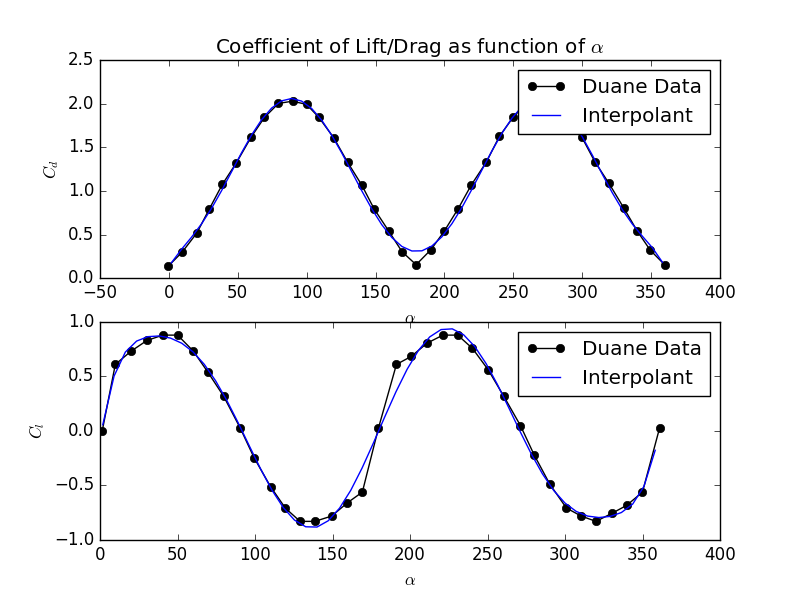
\includegraphics[width = 12 cm]{figs/flat}
    \caption{The flat plate interpolation.} 
    \label{flat}
  \end{center}
\end{figure}
As shown in Figure \ref{flat}, the fit is largely accurate to experimental data
as a point of comparison. 

At this point, we can calculate the force 
on the turbine as, 
\begin{equation}
 \boxed{F = \frac{1}{2}\frac{\rho u_p^2 C}{A}\left(C_l \cdot
					      n_\text{lift} + C_d \cdot n_\text{drag}  \right)}
\end{equation}

Where C is the chord length (specified as input), and A is the area,
which is also specified. For instance, the area swept might be, 
\begin{lstlisting}
     area_swept = '{r:=sqrt(x^2+y^2); 2*pi*r*(.6-.4)/4}'
\end{lstlisting}
for a 4 blade fan. The chord is specified similarly, for instance, 
\begin{lstlisting}
     chord_length = '.2*sqrt(2)'
\end{lstlisting}
would set a 0.28 meter chord length. 

Note that since GRINS is providing a volumetric forcing, 
the actual calculation will be of the form,

\begin{equation}
 \boxed{n F / 2 \pi r t = F'''}
\end{equation}
Where $t$ is the thickness of the turbine forcing region, and $n$ are the number of blades, 
or ''area swept``.